\documentclass[a4paper]{article}
\usepackage[margin=2.5cm]{geometry}
\usepackage{amsmath}
\usepackage{amssymb}
\usepackage{graphicx}
%opening
\title{Marking Correlation}
\author{Romain Lhotte \& Paul Dubois\footnote{both authors contributed equally to this work}}

\newcommand{\Var}[1]{\text{Var}\left( {#1} \right)}


\begin{document}
	\maketitle
	\begin{abstract}
		The evaluation of students' performance in higher education plays a crucial role in assessing the effectiveness of teaching methods and improving learning outcomes.
		In this study, we investigate the correlation between two teachers' grading practices in a deep learning course at the master's level, offered at CentraleSupélec.
		The two teachers, who have distinct teaching styles, were responsible for marking the final project oral presentation.
		Our results indicate a significant positive correlation between the two teachers' grading practices, suggesting that their assessments of students' performance are consistent.
		Although consistent with each other, grades do not seem to be fully reproducible from one examiner to the other.
	\end{abstract}
	
	\section{Introduction}
	In recent years, there has been a surge of interest in the field of deep learning, with applications ranging from computer vision and natural language processing to bio-informatics and medical diagnosis.
	As a result, there is an increasing demand for high-quality education and training programs in deep learning.
	In response to this demand, many universities and engineering schools have started offering courses and programs in deep learning at various levels, including undergraduate and graduate levels.
	
	This study focuses on the evaluation of a deep learning course offered to third-year engineering students at CentraleSupélec (Paris, France), who are pursuing the "Vivant, Santé, Environnement" (VSE) path.
	The course was designed to provide students with a comprehensive understanding of the fundamental concepts, theories, and applications of deep learning.
	The course was structured into 10 teaching sessions, each spanning three hours.
	Each session comprised one hour of theoretical instruction followed by two hours of practical exercises.
	In addition to the classroom instruction, five Kaggle challenges were assigned to the students, who were expected to work on them independently and outside of class time.
	The final component of the course consisted of a group project, which required the 28 students to form 10 groups of 2-4 individuals.
	The project served as a comprehensive assessment of the students' proficiency in deep learning and required the application of the concepts and techniques covered in the course.
	Students were expected to present their project findings orally and respond to questions from the instructors.
	
	The evaluation of students' performance in the course is a critical aspect of assessing the effectiveness of the teaching methods and the quality of the learning outcomes.
	In this study, we investigate the correlation between the grading practices of two instructors who taught the course, and the Kaggle assessments.
	Our goal is to evaluate the reliability and consistency of grading practices in higher education and to provide insights that can inform efforts to improve the quality of teaching and learning outcomes.
	
	The findings of this study have implications for educators, administrators, and policymakers who are interested in improving the quality of education in deep learning and related fields.
	The results can also be used to inform the development of more effective evaluation frameworks and grading practices in higher education.
	Overall, this study contributes to the growing body of knowledge on the pedagogy of deep learning and its applications in various fields.
	
	
	
	\section{Methods}
	\subsection{Participants}
	The participants in this study were 28 students enrolled in a deep learning course at the master's level offered at CentraleSupélec during the academic year 2022/2023.
	The class was taught by two instructors, both of whom had distinct teaching styles and backgrounds.
	
	\subsection{Evaluation Framework}
	The evaluation of students' performance in the course was based on six components, which accounted for the final grade.
	
	The first five components were Kaggle challenges, each accounting for 6\% of the total mark, adding up to 30\% of the final mark.
	For each challenge, a marking scheme was established, which was publicly shared with the students:
	\begin{itemize}
		\item [\textbf{3/6}] achieved a better score than one typically obtained after a \textbf{basic} attempt of the challenge
		\item [\textbf{4/6}] achieved a better score than one typically obtained after a \textbf{fair} attempt of the challenge
		\item [\textbf{5/6}] achieved a better score than one typically obtained after an \textbf{advanced} attempt of the challenge
		\item [\textbf{6/6}] given to the \textbf{top 10} students of the class; to obtain 6/6, students also needed to meet requirement for 5/6 (the class is 28 students, so this score is reachable for a third of the class)
		\item [\textit{0/6}] no attempt to the challenge or score \textit{below} what a typical \textit{basic} attempt of the challenge
	\end{itemize}
	Details on the exact scores level for each Kaggle challenges are explained in the supplementary material.
	
	The final component was a project, which accounted for the remaining 70\% of the final mark.
	Students completed the project in groups of 2-4, and the project was assessed based on an oral presentation of approximately 10 minutes, followed by approximately 10 minutes of questions.
	The final mark for the project was the average of the two independent marks given by the two instructors, who graded the projects separately.
	
	\subsection{Ethical Considerations}
	This study was conducted in accordance with the ethical guidelines of CentraleSupélec, and all participants were were anonymized for confidentiality purposes.
	%The study was approved by the institutional review board of CentraleSupélec?
	
	\subsection{Normalizing}
	The Kaggles were originally graded out of 6, the project out of 20.
	We normalized all graded to be out of 100 (\%), to ba able to compare mean and standard deviation.
	
	\section{Results}
	We rounded all numerical values to $10^-2$ for readability purposes.
	\subsection{Dependence of assessments}
	Suppose that the score of students on each kaggle were independent.
	Then probability theory tells us that the standard deviation of the average kaggle score should be $9.85$ (using $\Var{\frac{\sum_{i=1}^{5} K_i}{5}} = \frac{\sum_{i=1}^{5} \Var{K_i}}{5^2}$).
	However, the variance found is $13.22$.
	This means that the score on kaggle challenges are not independent of each others.
	It makes sense, since we expect good students to perform well in all assessments.
	
	Similarly, the variance of the project mark (average of the mark given by teacher 1 and 2) should be $6.95$ (using $\Var{\frac{P_1 + P_2}{2}} = \frac{\Var{P_1} + \Var{P_2}}{2^2}$) if the two teachers marked as independent random variables.
	However, we observe a variance of $9.13$, leading to the conclusion that the two teachers marks cannot be treated as random independent variables.
	Again, this is expected, since teachers do not mark randomly (most of the time).
	
	\subsection{Distribution of the marks}
	We can plot the Kernel Density Estimate (KDE) for the distribution of the marks, both for Kaggle challenges and for the project:
	\begin{figure}
		\centering
		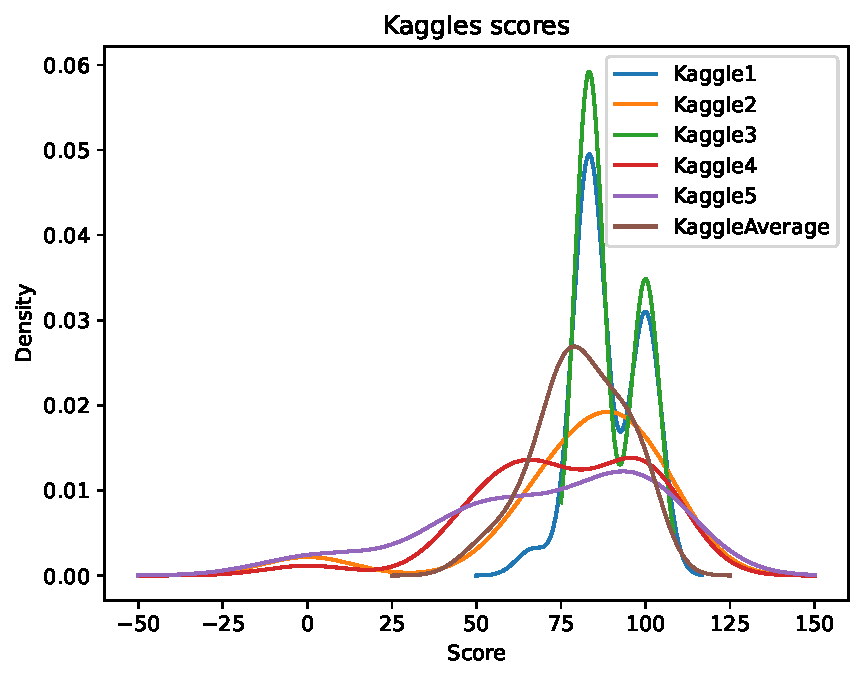
\includegraphics[width=0.49\textwidth]{figures/kaggles_densities.pdf}
		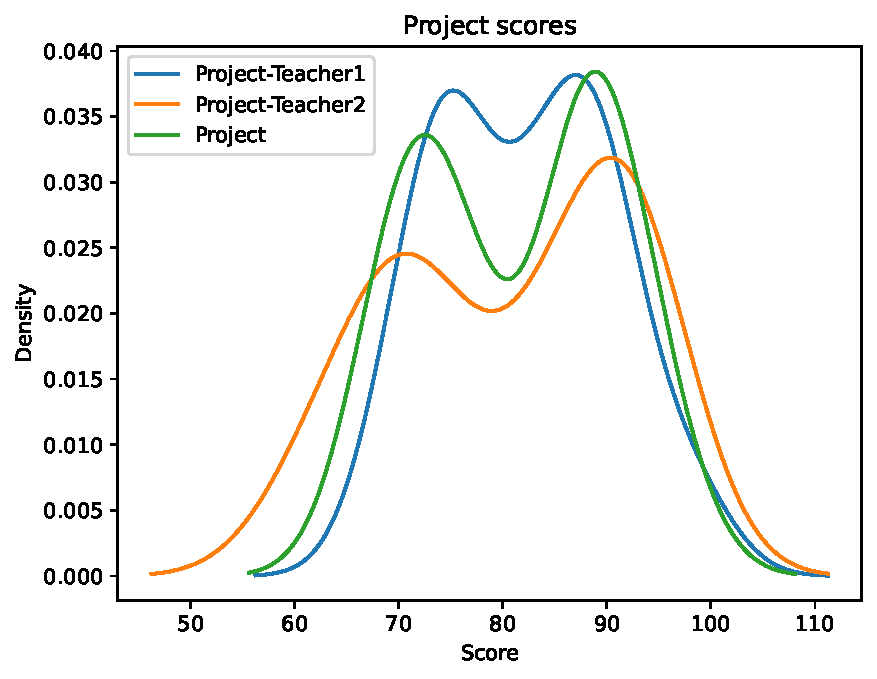
\includegraphics[width=0.49\textwidth]{figures/project_densities.pdf}
		\caption{KDE}
		\label{fig:KDE}
	\end{figure}
	We observe that the class splits into two groups: one achieving nearly perfect score, and one getting about 75\%.
	This trends can be observed in the project scores given by teachers 1 and 2, but also on some of the kaggle challenges: (kaggles 1 and 3 where it's obvious to observe, and kaggle 4 and 5 where it's less sharp).
	
	\subsection{Quantification of the inter assessments correlation}
	\section{Discussion}
	\section{Conclusion}

\end{document}
